\documentclass[tikz,border=5pt]{standalone}
\usepackage{tikz}
\usetikzlibrary{arrows.meta,decorations.pathmorphing}
\definecolor{nebula}{HTML}{6366F1}
\definecolor{spark}{HTML}{14B8A6}
\definecolor{ink}{HTML}{334155}
\begin{document}
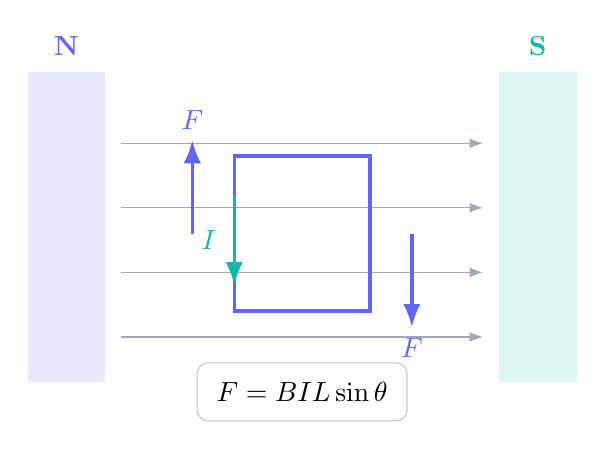
\begin{tikzpicture}[font=\sffamily,>=Latex,x=.82cm,y=.82cm]
  \fill[nebula!14] (0,0) rectangle (1.2,4.8);
  \fill[spark!14] (7.3,0) rectangle (8.5,4.8);
  \node[text=nebula,font=\bfseries] at (.6,5.2) {N};
  \node[text=spark,font=\bfseries] at (7.9,5.2) {S};
  \foreach \y in {.7,1.7,2.7,3.7}{\draw[->,ink!45] (1.45,\y)--(7.05,\y);}
  \draw[very thick,nebula] (3.2,1.1) rectangle (5.3,3.5);
  \draw[->,very thick,spark] (3.2,2.9)--(3.2,1.5) node[midway,left=5pt,fill=white,inner sep=1pt] {$I$};
  \draw[->,very thick,nebula] (2.55,2.3)--(2.55,3.75) node[above] {$F$};
  \draw[->,very thick,nebula] (5.95,2.3)--(5.95,.85) node[below] {$F$};
  \node[draw=ink!30,rounded corners=4pt,fill=white,inner sep=7pt] at (4.25,-.15)
    {$F=BIL\sin\theta$};
\end{tikzpicture}
\end{document}
